\chapter{Planning and learning with Tabular methods}
\section{Summary}

\subsection{Models and planning}
Planning uses a model of the System, while learning uses experience.

There are 2 major types of planning
\begin{enumerate}
	\item State space planning
	\item Plan space planning (for example genetic programming)
\end{enumerate}

\subsection{Dyna: integrated planning an learning}

A value function/policy leads to an action, this results in experience that can directly improve the value/policy via reinforcement learning. It can also be used to improve a model of the system. A plannings algorithm can then improve the policy/value function via the model. This is illustrated in figure~\ref{fig:dyna flow}.

\begin{figure}
\centering
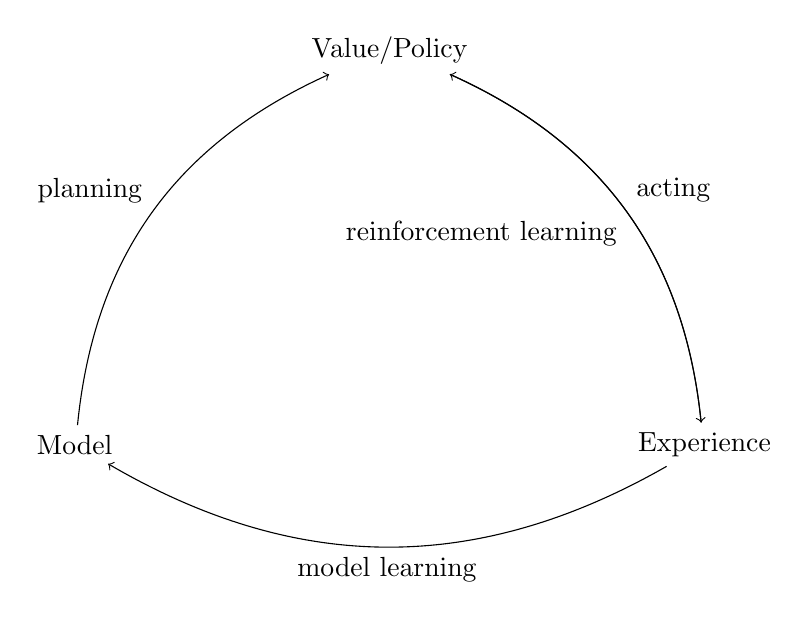
\begin{tikzpicture}

\node at (4, 0) (a) {Value/Policy};
\node at (8, -5) (b) {Experience};
\node at (0, -5) (c) {Model};

\draw [->, auto, bend left] (a) to node {acting} (b);
\draw [->, auto, bend left] (b) to node {model learning} (c);
\draw [->, auto, bend left] (c) to node {planning} (a);
\draw [->, auto, bend right] (b) to node {reinforcement learning} (a);
\end{tikzpicture}
\caption{Dyna}
\label{fig:dyna flow}
\end{figure}

\textbf{Dyna Q} is an example of a Dyna algorihm. It uses Q-learning on the experience to improve the value function. Saves the state/action pair with the result. And then uses Q-learning on the model(table) to further improve the value function.

\subsection{When the model is wrong}
If the optimal path is suddenly significantly worse then before, it takes quiet a while to adjust with Dyna. But even worse is when a better path suddenly becomes available, as Dyna has no reason to look for it. It might stay undiscovered.

DynaQ+ Tries to asses this weakness by adding a bonus reward on each state in the value function when planning. $r + k \sqrt{\tau}$, where $r$ is the normal simulated reward, $k$ is a small number (parameter), and $\tau$ is the number of step since the last visit.

\subsection{Prioritized sweeping}


Prioritized sweeping is a form of planning called \textbf{backward focusing}. When a state value changes, it identifies the predecessor states and the change in value function. It puts them on a queue, ordered according to their value function change. The state with the highest change then gets the same treatment. 


The opposite approach would be \textbf{forward focusing} which updates all the successors of a state that has a value change.

\subsection{Expected vs Sample updates}
Value function updates have 3 binary dimensions:
\begin{center}
\begin{enumerate}
	\item state vs action value function
	\item estimated using arbitrary policy or optimal policy
	\item expected vs sample update
\end{enumerate}
\end{center}

This sums up to 8 possible combinations illustrate in table~\ref{tab:table of one step updates}.

\begin{center}
	\begin{table}[H]
	\begin{tabular}{ c | c | c }
		value estimation & expected updates & sample updates \\
		\hline
		$v_\pi$ & policy evaluation & TD(0) \\ 
		$v_*$ & value iteration & \\  
		$q_\pi(s, a)$ & q-policy evaluation & sarsa \\
		$q_*(s, a)$ & q-value iteration & Q-learning	
	\end{tabular}
	\label{tab:table of one step updates}
	\caption{table of one step updates}
	\end{table}
\end{center}

The \textbf{expected update} is equation~\ref{eq:expected update for state action pair} uses $\hat{p}$ the estimated dynamics of the system to estimated the probability of getting a certain state with a certain result. 

The \textbf{sample update} from equation~\ref{eq:sample update for state action pair} doesn't need a model as updates with the actual state/action and reward applied to the system. This makes the sample update a lot less computational expensive.

If the system only has 1 possible next state, then the expected and sample update are the same. However once there is more then 1 possible next state, there is a \textbf{sample bias} on the sample updates.

The error of the sample update drops with $\sqrt{\frac{b-1}{bt}}$, where $b$ is the branching factor, the number of possible next states $s'$ for which $\hat{p}(s'|s,a)>0$). And $t$ the number of sample updates. This formula suggests that \textbf{sample updates are good with system with large branching factors}. 

\begin{equation}
Q(s, a) = \sum_{s', r} \hat{p}(s', r| s, a)[r + \gamma \max_{a'}Q(s', a')]
\label{eq:expected update for state action pair}
\end{equation}

\begin{equation}
Q(s, a) = Q(s, a) + \alpha[R + \gamma \max_{a'}Q(S', a') - Q(s, a)]
\label{eq:sample update for state action pair}
\end{equation}

\subsection{Trajectory Sampling}

In dynamic programming there are 2 way's to distribute updates of the value function. Either \textbf{exhaustively} in 1 sweep, or \textbf{according to some distribution}.

On-policy learning \textbf{$\epsilon$-greedy will converge very fast}, as it skips a large part of the irrelevant state space. It will however not converge to the actual value in the long run, but will have some sample bias. 

\subsection{Real-time dynamic programming}

RTDP is an on-policy trajectory sampling value iteration algorithm.

RTDP can find optimal policies without infinitely visiting all states. It's very good with big and stochastic problems.

\subsection{Planning at decision time}

The planning phase of an DP algorithm can happen on the background, this is called \textbf{background planning}.

Decision time planning only does the planning when a new state change occurs. It's less accurate, but has very fast response times.

\subsection{Heuristic Search}

Heuristics have man made value functions, they look at the now, so no simulations.

\subsection{Roll-out algorithms}

Decision-time planning based on Monte Carlo Control. They estimated the action values from the current state by simulating trajectories from the current state. And when the action value is accurate enough it applies the action. And forgets all the past runs. The simulations itself can be run in parallel.

The name \textbf{rollout} comes from the game backgammon. Roll-out algorithms were studied on backgammon games, the algorithm would randomly select dice rolls and play out the game.

\subsection{Monte Carlo tree search}

A \textbf{tree policy} keeps track of value function via tree of state/action values. It executes \textbf{monte carlo} simulations at the leafs of the trees to get return values to update the tree. 

It's a \textbf{roll-out} algorithm as it starts from 1 specific state, and forgets everything after an action was taken.  \textbf{decision time planning}. (although some information could be reused for the next tree)

There are 4 major steps:

\begin{enumerate}
	\item Selection: A tree policy based on action values on the tree selects a leaf node
	\item Expansion: Potentially the tree could be expanded with a new leaf by the tree policy
	\item Simulation: A roll-out policy simulates to the end of the episode
	\item Backup: The return value of the roll-out episode is backup-ed into the action values of the tree.
\end{enumerate}

\section{Exercises}

\subsection{Exercise 8.1}
A Dyna method can do much better then a multi-step method. If the path is longer then the horizon of the multi-step method. The Dyna method can propagate the end result over the entire path. While the multi-step method is limited to it's horizon.

\subsection{Exercise 8.2}
Dyna+ will get good rewards on previously bad states if that state was not visited for a while. Pushing the algorithm to re-visit it from time to time. The parameter $k$ controls how much exploration Dyna+ needs to do.

\subsection{Exercise 8.3 page 168}
Dyna and Dyna+ had bad rewards on the previously good path. So relatively speaking older not so good states are getting better. Dyna+ accelerates this effect by also adding the bonus reward.

\subsection{Exercise 8.4 page 168}
programming task TODO

\subsection{Exercise 8.5 page 168}
The algorithm should keep updating it's value function, but it might be a good idea to use a moving average. The moving average will help with the stochastic environment, but will will make the change environment worse. So a trade-off on the window size should be made. 

\subsection{Exercise 8.6 page 174}
If some new states are much more likely then others, then sample updates will work a lot better. As the very likely transitions will be the most influential on the behavior of the system, and due to be likely will also be very present in the sample updates. 

\subsection{Exercise 8.7 page 177}
We observe $b$ goes up, the lines get smoother. When $b$ is very low, one good sample update can significantly improve things. While if $b$ is large, the optional actions are more spread out as the next state $s'$ is more stochastic. So you can only improve it on average. (not sure about this)

\subsection{Exercise 8.8 page 177}
progamming TODO
